\section{Caso pratico: La Posta}
Come anticipato nell’introduzione La Posta è il miglior esempio, in Ticino di automazione in larga scala. I temi trattati in questo capitolo sono i seguenti: le nuove tecnologie e la chiusura degli uffici postali. Le principali informazioni provengono dai comunicati stampa della Posta disponibili sul sito ufficiale, dall’intervista con il sindacato della Posta Syndicom (nella figura di riferimento di Marco Forte che è il responsabile regionale) e dal libro di Graziano Pestoni intitolato “La privatizzazione della Posta svizzera”.

\subsection{La Posta in breve}
La Posta nasce nel 1849 ed è tutt’ora proprietà della Confederazione nonostante la sua trasformazione in società anonima avvenuta nel 2013.

\subsubsection{La privatizzazione}
La Posta è stata separata dalle Telecomunicazione, ciò significa che non riceve più sussidi che permettevano alla Posta di offrire servizi di qualità e di coprire i disavanzi con gli utili delle telecomunicazioni. La Posta è stata trasformata in un primo tempo in azienda autonoma e in seguito in società anonima. Invece, le telecomunicazioni sono state da subito trasformate in società anonime e il capitale è stato ceduto ai privati.
La Posta e le Telecomunicazioni non stanno più funzionando come aziende pubbliche, ma come qualsiasi azienda privata. L’obbiettivo sembrerebbe non essere più quello di fornire il miglior servizio possibile al minor costo possibile, ma nel realizzare risultati finanziari positivi.

\subsubsection{La liberalizzazione (apertura del mercato alla concorrenza}
Il volume dei pacchi e il servizio degli espressi è in costante e forte aumento in seguito allo sviluppo dell’e-commerce (vendita per corrispondenza). È un settore altamente redditizio ed è per questo motivo che in diversi Paesi è stato liberalizzato. Questo significa che il mercato è caratterizzato dalla presenza dell’operatore storico (ex servizio postale nazionale) e da aziende private e si crea così un clima di concorrenza all’interno di esso. Inoltre il volume delle lettere distribuite sta subendo una diminuzione costante in seguito alla concorrenza esercitata dalle nuove tecnologie, in particolare dalla posta elettronica.
\subsection{Integrazione nuove tecnologie (innovazioni)}
Per la Posta è importante sviluppare continuamente nuove soluzioni sia fisiche che digitali per semplificare la vita quotidiana dei clienti. All’interno della Posta è stata creata nel 2014 un’unità operativa che si occupa dello Sviluppo e delle Innovazione, per questo motivo la Posta segue attivamente gli sviluppi, le opportunità commerciali e le tendenze sviluppando nuovi modelli operativi. L’azienda sta sperimentando e integrando l’impiego di nuove tecnologie come droni, robot di consegna e navette senza conducente. In questo modo la Posta riesce a stare al passo con i tempi e riconosce le potenziali esigenze della clientela modificando la sua attività di base.
\begin{figure}
    \centering
    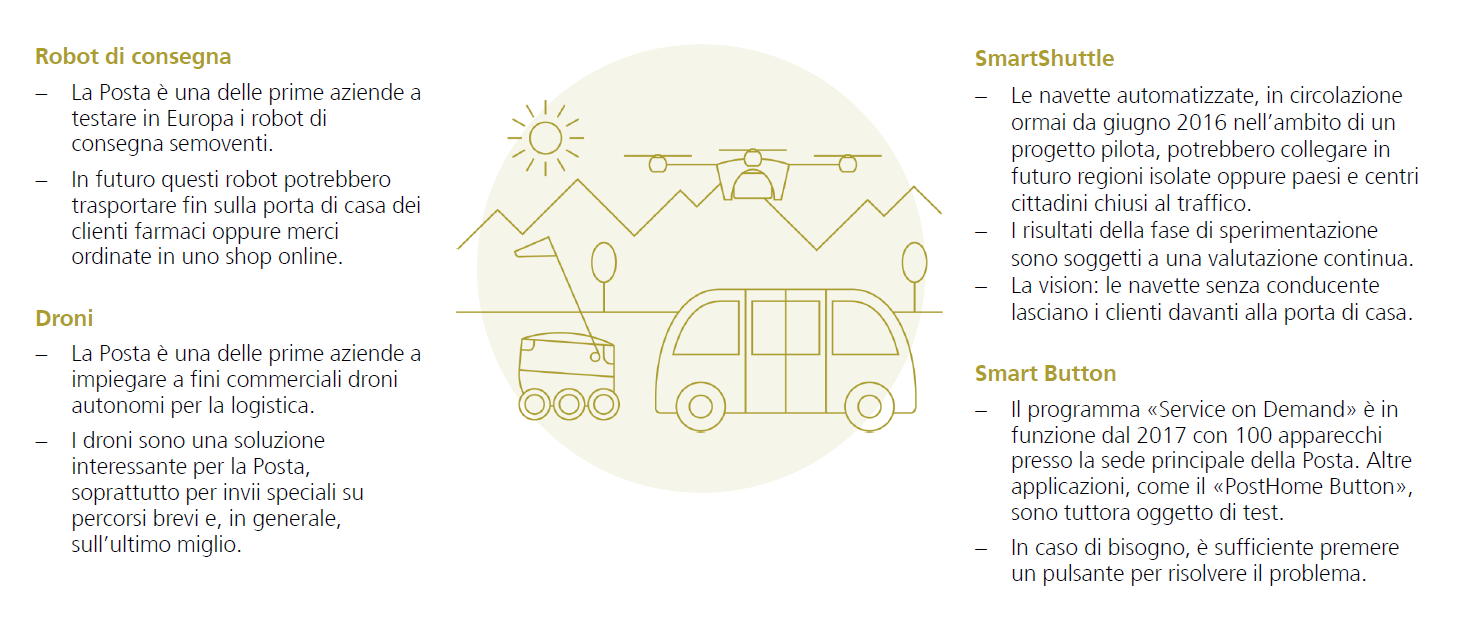
\includegraphics{sviluppi.PNG}
    \caption{Caption}
    \label{fig:my_label}
\end{figure}

\subsubsection{In Svizzera}
Nel comunicato stampa (01.06.2015) pubblicato sul sito ufficiale della Posta intitolato “La Posta installa sportelli automatici per i pacchi presso le stazioni FFS” viene riportata la decisione della Posta di installare nelle stazioni FFS gli sportelli automatici My Post 24. Questa decisione avviene per stimolare una partnership strategica e per favorire le operazioni di ricezione e impostazione dei pacchi dei clienti. 
Nel comunicato stampa (13.10.2017) pubblicato sul sito ufficiale della Posta intitolato “Nuovi impieghi per i robot di consegna della Posta” viene riportato che il gigante giallo sta testando l’impiego di robot di consegna nel centro di Zurigo (circa 170 consegne effettuate). La Posta intende impiegare i robot in ulteriori attività logistiche in altre località. 
Nel comunicato stampa (04.12.2018) pubblicato sul sito ufficiale della Posta intitolato “Un drone della Posta trasporterà campioni di laboratorio tra l’Ospedale universitario e l’Università di Zurigo” viene riportato il progetto che durerà un anno. I droni autonomi trasporteranno i campioni di laboratorio dall’Ospedale universitario di Zurigo (USZ) alla sede di Irchel dell’Università di Zurigo (UZH). Il punto cardine del progetto è la differenza tra il trasporto aereo rispetto a quello su strada, infatti i droni raggiungono la destinazione nella metà del tempo avvantaggiando i pazienti, i medici e il personale infermieristico. 
Nel comunicato stampa (26.01.2018) pubblicato sul sito ufficiale della Posta intitolato “Robot di consegna: bilancio positivo della Posta per i test eseguiti a Dübendorf” viene riportato l’esperimento svolto dal gigante giallo per consegnare i pacchi con l’ausilio di robot. Infatti il robot ha percorso nella fase di test 800 chilometri senza incidenti o imprevisti e le 200 corse hanno permesso alla Posta e al costruttore di acquisire importanti informazioni. Nel documento viene posto l’accento sulle necessità dei clienti, che sono sempre più mobili e vorrebbero ricevere la merce ordinata il prima possibile, e sulle reazioni delle persone all’impiego di robot per la consegna dimostrando che c’è interesse e curiosità verso il tema. 
\subsubsubsection{In Ticino}
Nel comunicato stampa (04.10.2017) pubblicato sul sito ufficiale della Posta intitolato “I droni tornano a volare a Lugano” viene riportato il collegamento di droni tra due ospedali di Lugano che trasporteranno campioni di laboratorio o farmaci urgenti.  È la prima volta che vengono impiegati i droni per questa tipologia di scambio, una prima svizzera che vede la Posta pioniera nell’ambito della logistica con i droni anche a livello mondiale. 
\subsubsection{Confronto}
Mettendo a confronto le innovazioni tecnologiche effettuate dalla Posta in Ticino e nel resto della Svizzera, si nota chiaramente che sono nella maggior parte testate e introdotte nel resto del paese per una serie di motivi che sono legati alla situazione economica ticinese, alla morfologia del territorio e alla concentrazione di start up innovative.
\subsection{Richiesta dati}
Negli allegati potrete trovare una lettera di richiesta dati che nei giorni scorsi ho inviato alla Posta. I dati da me richiesti fanno riferimento al numero di impiegati presso la Posta in Svizzera e in Ticino e all’andamento delle assunzioni e dei licenziamenti per l’anno 2014. In questo modo si possono confrontare con i dati della disoccupazione presi dal rapporto di sintesi “Ai margini del mercato del lavoro” e ritrovare nelle possibili cause l’avvento della quarta rivoluzione industriale. Infine ho chiesto i dati relativi al numero di impiegati per le nuove forme di lavoro riportate nel dossier tematico “Nuove forme di lavoro per un mondo in continua evoluzione” elaborato dalla Camera di Commercio all’interno del quale vengono inoltre riportati i risultati di un recente studio europeo (Eurofound). L’obiettivo è di collegare concretamente il caso sulla Posta alla prima parte del dossier più teorica in modo diretto con l’elaborazione dei dati richiesti. Sfortunatamente ho ricevuto una risposta negativa, la Posta non può rilasciare questi dati sensibili, pertanto non potrò concretizzare l’analisi che mi ero inizialmente prefissata.
\subsection{Altri attori coinvolti}
\subsubsection{Stato}
La Posta deve sottostare alla Legge federale sull’organizzazione della Posta Svizzera (LOP). 
Lo Stato sta intervenendo legiferando e ponendo un limite alle aziende per quanto riguarda l’integrazione delle nuove tecnologie. Per quanto riguarda La Posta lo Stato ha posto un numero minimo di impiegati agli sportelli. Diversi stati stanno applicando questo tipo di leggi per cercare di tutelare i lavoratori.

\subsubsection{Sindacato}
Il sindacato di riferimento per La Posta e per altre aziende che come lei operano nel settore della comunicazione è Syndicom.
Nell’articolo “Il Consiglio nazionale dorme e la Posta racconta bugie- Un appello al Gran Consiglio” redatto da Syndicom viene alzata una critica al Gran consiglio del Cantone Ticino che il 12 dicembre 2016 accolse una risoluzione volta ad adottare una minatoria sulle chiusure degli uffici postali. Il Consiglio federale e la direttrice del DATEC, Doris Leuthard, fecero sapere che la minatoria non è necessaria. A seguito della situazione creatasi il Consiglio di amministrazione e la direzione della Posta hanno continuato a chiudere gli uffici postali situati sul territorio ticinese. La critica continua questa volta rivolta alle filiali in partenariato che secondo il sindacato non offrono ciò che la Posta sostiene: i servizi sono gli stessi e gli orari non sono più estesi, quest’ultimi avranno la stessa durata dei normali uffici postali. Sempre secondo Syndicom il servizio rischia solo di peggiorare e i clienti non potranno effettuare le usuali operazioni che fino ad ora erano svolte attraverso l’ufficio postale. Un altro aspetto da considerare secondo il sindacato è la formazione del personale, infatti i buralisti postali ricevono una formazione di due anni, mentre i responsabili di filiali in partenariato di soli due giorni. Malgrado il segreto professionale, si sollevano dubbi sulla privacy dei pagamenti, dell’invio o del ritiro di raccomandate o di altre operazioni delicate. Il discorso prosegue ribadendo l’inadeguatezza degli orari di apertura degli uffici postali rimanenti che vengono ridotti per contenere i costi di esercizio continuando a sostenere che l’utenza negli uffici postale sta diminuendo in quanto i clienti preferiscono effettuare le operazioni online. 
L’intervista a Marco Forte che è il responsabile regionale per il Ticino e Moesano ha fatto emergere che il sindacato è critico nei confronti del Parlamento, in quanto sono in corso delle iniziative e delle mozioni che non sono state ancora votate. La moratoria il cui scopo è quello di sospendere la chiusura degli uffici postali ne è un chiaro esempio. Come sindacato chiedono l’intervento della politica perché gli unici che possono fermare questo smantellamento sono i politici a Berna.

\subsubsection{Fenomenti esterni}
Sempre più le persone tendono a interagire tra loro attraverso la posta elettronica, a pagare con sistemi online (es. e-banking, PayPal, addebito diretto, ecc.) e spesso i pacchi che arrivano a casa non sono consegnati tramite la posta, ma attraverso altri intermediari.
La Posta risente di questi fenomeni legati alla globalizzazione e alla facilità di accesso e alla gratuità di Internet, per questo motivo cerca di stare al passo e di sopravvivere effettuando delle scelte strategiche come investire nell’automatizzazione e chiudendo gli sportelli perché obsoleti e di nicchia per coloro che sono contro tendenza rispetto ai tempi.
Il gigante giallo si rende conto che le abitudini dei suoi clienti stanno cambiando: si rivolgono sempre meno all’ufficio postale tradizionale, ma svolgono le operazioni sullo smartphone o con il computer con una possibilità di accesso 24 ore su 24. La Posta reagisce quindi cercando di puntare su un mix di punti di accesso digitali e fisici su misura per le esigenze locali. Da qui la conseguente e massiccia chiusura degli sportelli in svariati comuni del Cantone.

\subsection{Chiusura degli sportelli}
Nell’articolo “La rete postale del futuro” pubblicato sul sito ufficiale della Posta si riporta l’impegno da parte sua di sviluppare entro il 2020 la rete postale con più di 4’200 punti di accesso in Svizzera, puntando sulle filiali partner, sul servizio a domicilio, sugli sportelli automatici MyPost 24 e altri punti di impostazione e di ritiro. 
Un dialogo con la politica (Comuni e Cantoni) e i cittadini è fondamentale per definire le esigenze regionali e rendicontare le proprie azioni garantendo la trasparenza, la sicurezza della pianificazione e ottenere l’approvazione dagli stakeholder.

\subsubsubsection{Obbiettivi strategici del Consiglio Federale}
Fra questi obbiettivi (vedi “Presentazione aziendale della Posta” in allegato) vi è quello di aumentare a lungo termine il valore aziendale e i suoi rendimenti. Questo porta la Posta a ragionare in termini di costi al punto da giustificare la chiusura quasi sistematica degli uffici postali.
\subsubsection{Procedura di chiusura o di trasformazione}
Se la Posta intende chiudere o trasferire un ufficio o un’agenzia postale, deve dapprima consultare l’autorità competente del Comune interessato e cercare di trovare una valida soluzione alternativa.
Se tra le parti non si giunge a un consenso comune, entro 30 giorni dalla notifica della decisione della Posta il Comune può adire la PostCom, la quale verifica se:
\begin{itemize}
    \item la Posta ha consultato il Comune interessato, cercando di trovare una soluzione consensuale;
    \item la decisione tiene conto delle particolarità regionali;
    \item anche dopo l’attuazione della decisione il 90\% della popolazione può raggiungere la rete postale in 20 minuti (a piedi o con i mezzi pubblici);
    \item nella regione interessata rimane aperto almeno un ufficio postale.
\end{itemize}
Entro sei mesi dall’inoltro del ricorso oppure in seguito a una procedura di conciliazione, la PostCom rilascia una raccomandazione all’attenzione della Posta. Fino a quel momento la Posta non può procedere alla chiusura o al trasferimento. La Posta decide in via definitiva tenendo conto della raccomandazione della PostCom.
Il sindacato muove una critica contro il potere decisionale della Posta che annulla la volontà del sindaco e dei cittadini, come afferma anche Marco Forte: \textit{“In realtà il sindaco non può decidere nulla perché in pratica può solo decidere dove posizionare l’agenzia, ma di fatto della chiusura non è una discussione che la Posta fa con il municipio, quindi impone le chiusure e questo perché la legge glielo permette. La Posta ha sempre l’ultima parola, quindi anche se il sindaco e i cittadini raccolgono le firme per le petizioni e dimostrando il loro disaccordo, la Posta chiude lo stesso.”}

\subsubsection{In Ticino}
L’obbiettivo della Posta è quello di trovare un mix ideale tra filiali proprie, filiali in partenariato, punti di accesso per i clienti commerciali e il collocamento di punti di impostazione e di ritiro integrativi.
La Posta sta definendo il futuro delle restanti filiali della Posta finora non garantite. Le filiali in partenariato stanno giocando un ruolo importante nel destino delle restanti, infatti il vantaggio sta nell’offrire ai clienti un’offerta postale ampia, orari di apertura interessanti e rafforzare il rapporto di collaborazione con partner locali (infrastrutture presenti all’interno del paese o del quartiere).
L’intenzione della Posta è quella di chiudere le filiali offrendo valide alternative.
Dall’intervista con Marco Forte è emerso che i collaboratori della Posta godono di un buon contratto sociale tra le parti, ma questo non è più sufficiente visto la massiccia chiusura degli uffici postali e l’avvento dei licenziamenti definiti come “licenziamenti tecnologici, dovuti quindi dalla sostituzione dell’uomo dalle macchine. Le persone che gestiscono le filiali in partenariato non sono impiegate direttamente dalla Posta e di conseguenza non sottostanno al contratto collettivo. In futuro molto probabilmente il numero di persone che non avranno più un posto di lavoro presso la Posta aumenterà considerevolmente proprio a causa delle continue chiusure degli uffici perché non sarà più possibile mantenere tutti i posti all’interno dell’azienda.
Per quanto riguarda i licenziamenti dei collaboratori a causa della chiusura delle filiali La Posta afferma di fare il possibile per evitarli, di elaborare soluzioni volte a salvaguardare l’impiego del personale e prevede le seguenti misure:
\begin{itemize}
    \item creazione di una borsa lavoro (offerte di lavoro all’interno della Posta);
    \item corsi di formazione e perfezionamento mirati;
    \item outplacement per soluzioni al di fuori della Posta;
    \item negoziazione con i sindacati.
\end{itemize}
L’intervento dei sindacati si è già tuttavia reso necessario, come riporta Marco Forte. Inoltre constata che nonostante la Posta dica di evitare i licenziamenti, non sta rallentando la chiusura degli uffici postali che implica una soppressione di posti di lavoro che l’azienda non è in grado di reintegrare al suo interno. Nel resto della Svizzera si sta verificando la stessa situazione, la Posta sta effettuando licenziamenti in tutto il Paese. La chiusura degli uffici postali è un problema importante.
Negli ultimi due anni il numero di punti di accesso in cui i clienti possono usufruire dei servizi postali sono 1’033 in tutta la Svizzera. Dal 2016 sono stati condotti oltre 550 colloqui con autorità cantonali e comunali e La Posta ha organizzato oltre 270 eventi informativi per la popolazione. Con un investimento di circa 40 milioni di franchi La Posta intende modernizzare circa 300 filiali gestite in proprio in tutta la Svizzera, consolidare la rete con altri 200 sportelli automatici MyPost 24 e con stazioni self-service attualmente in fase di test.
Secondo il sindacato la Posta non agisce in modo trasparente e fuorvia con una comunicazione e una espressione poco chiara. Nell’intervista Marco Forte ha affermato che \textit{“Per quanto riguarda gli uffici postali per molti collaboratori c’è stata una diminuzione del 10\% dell’impiego in tutto il Ticino. Questa diminuzione è causata dalla chiusura degli uffici postali e dalla produttività. La Posta con il termine produttività intende dire che non ci sono abbastanza clienti per il personale presente, ciò è dovuto alla chiusura dell’ufficio postale, perché il personale viene trasferito in un altro ufficio. È chiaro che poi il personale aumenta e secondo la Posta c’è troppo personale rispetto al lavoro.”} La diminuzione del 10\% del lavoro è un ottimo spunto di riflessione perché è anche strettamente legato alla quarta rivoluzione industriale come dimostra questa testimonianza anonima di un impiegato della Posta:
\textit{“L’impianto automatizzato di Cadenazzo ha la funzione di smistare le lettere e i pacchi per ordine di consegna. Nelle filiali di distribuzione arrivano i camion con la posta da consegnare già smistata. Questo impianto toglie una gran parte del lavoro che solitamente ero tenuto a svolgere. Prima di questa automazione il compito di smistare la Posta era il mio e mi prendeva buona parte del tempo di impiego e così riuscivo a coprire le 8h di lavoro. Oggi invece il mio lavoro si riduce a 2h e non ho lavoro per le restanti 6h, ma sono comunque obbligato a restare sul posto di lavoro e non posso permettermi di farmi vedere dai capi con le mani in mano, ma questo ragionamento lo fanno tutti i dipendenti. Tra i collaboratori della Posta si è creato un clima teso, una volta non era così si aveva molto più lavoro, ma lo si prendeva con un’altra filosofia.”}
È evidente che i lavoratori sono i primi che vivono sulla propria pelle e a proprie spese la quarta rivoluzione industriale. Oggigiorno alle nostre latitudini non tutte le aziende stanno integrando le nuove tecnologie, perché non tutte hanno i mezzi necessari per farlo. La situazione qui riportata è l’esempio di quello che sta accadendo sempre più spesso all’interno delle grandi aziende del territorio e nel mondo. Finché la situazione non sarà la medesima per tutti i collaboratori e il fenomeno diverrà fin troppo evidente, le aziende e lo Stato difficilmente interverranno a difenderli. Il sindacato della Posta ha già mosso due soluzioni interessanti e che vanno in questa direzione. La prima consiste in una riduzione del tempo di impiego che però la Posta non ha accettato, mentre la seconda consiste in una distinzione tra i licenziamenti tradizionali e quelli tecnologici con la conseguente creazione di due fondi separati. Un’osservazione interessante sollevata da Marco Forte è la seguente: le macchine porteranno a profitto le aziende e quest’ultimo deve andare a beneficio dei cittadini. Qui si evidenziano dei concetti che sono fondamentali per trovare una conciliazione tra uomo e macchine:
\begin{enumerate}
    \item \textbf{Part-time} come soluzione alla diminuzione del tempo di impiego e attraverso i turni e le alternanze dei collaboratori l’azienda può coprire molto di più delle tradizionali 8h lavorative.
    \item \textbf{Leggi} atte a tutelare i collaboratori dal licenziamento tecnologico e che obbligano le aziende che impiegano le nuove tecnologie ad assumere un minimo di lavoratori.
    \item \textbf{Reddito di cittadinanza} che è costituito per una buona parte dai profitti delle aziende tecnologiche e che di conseguenza permetterebbe alle stesse aziende di diminuire i salari di rendere così la manodopera attrattiva rispetto alle macchine.
\end{enumerate}
Se in questo periodo di transizione le persone si impegnano affinché vengano elaborate e progressivamente introdotte queste soluzioni la quarta rivoluzione industriale rappresenterà un punto di svolta per tutti e non per pochi.
La quarta rivoluzione industriale è sospinta principalmente dalle aziende, come ad esempio la Posta che è la prima a sollecitare i propri clienti per andare verso la digitalizzazione e quindi all’uso dell’E-commerce e dell’E-banking. Le aziende, quindi sono a favore dell’avvento della quarta rivoluzione industriale, perché vantaggiosa a livello economico, ma allo stesso tempo non si assumono la responsabilità di queste pressioni verso i collaboratori e la società nel suo insieme e non lo faranno fin tanto che la politica intervenga emanando delle leggi che indicheranno le modalità di applicazione delle misure risolutive sopra citate.  
Nell’articolo intitolato “La Posta: 61 uffici postali in Ticino almeno fino al 2020” vengono riportate le strategie della Posta per la rete postale del futuro. Una parte della strategia consiste in un dialogo con i rappresentanti della politica e dell’economia e con la popolazione per far fronte alle esigenze regionali e alla futura configurazione della rete postale. Per il momento 61 Uffici postali saranno mantenuti fino al 2020 mentre altri 48 sono a rischio. La Posta lavorerà alla creazione di 17 ulteriori punti di accesso offrendo punti clienti commerciali, punti di impostazione e di ritiro e il collocamento degli sportelli automatici MyPost 24 nelle maggiori località del Cantone. Le filiali in partenariato sono per la Posta molto vantaggiose in quanto permettono di offrire ai clienti un’offerta postale ampia e orari di aperture interessanti rafforzando l’infrastruttura presente nel paese o nel quartiere, in collaborazione con i partner locali. La Posta eviterà dialogando con i comuni di chiudere gli uffici postali senza presentare valide alternative. Il gigante giallo offrirà nuovi servizi come ad esempio per i clienti residenti in località che dispongono di una filiale in partenariato ci sarà la possibilità di effettuare versamenti in contanti sulla porta di casa; nelle località senza recapito mattutino, verranno consegnati i quotidiani in abbonamento fino a mezzogiorno; saranno offerte nuove soluzioni per le PMI che effettuano pagamenti in contanti e all’impostazione e il ritiro di invii. 

\subsubsection{Operazioni allo sportello in netto calo}
Secondo un’analisi svolta dalla Posta sull’affluenza di clienti agli sportelli è in netto calo. La Posta sostiene che la struttura obsoleta della rete genera costi elevati e che invece la ristrutturazione della rete postale ha portato risultati positivi riducendo il deficit di bilancio. A sostegno della riforma si riscontra un drastico calo del numero dei pacchi (-44\%) e di lettere (-68\%) e delle prestazioni nel traffico dei pagamenti (-44\%) allo sportello dal 2000. La trasformazione della rete si rende quindi necessaria per offrire ai clienti maggiori e migliori opportunità per effettuare le proprie operazioni postale e contribuisce a ridurre il deficit della rete postale.
\begin{figure}[h]
    \centering
    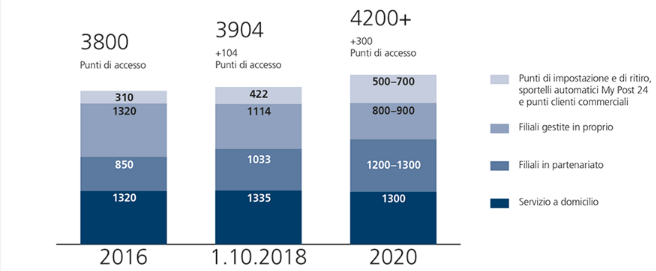
\includegraphics{Affluenza sportelli.PNG}
    \caption{Caption}
    \label{fig:my_label}
\end{figure}

\subsubsection{Abitudini della clientela}
\textbf{Evoluzione numero uffici postali}
\begin{table}[h]
\begin{tabular}{|l|l|l|l|l|l|l|}
\hline
Anno   & 1970  & 1999  & 2005  & 2010  & 2016  & 2020 \\ \hline
Uffici & 4'100 & 3'476 & 2'379 & 1'944 & 1'323 & 800  \\ \hline
\end{tabular}
\end{table}
La Posta sostiene di essere attenta e di tenere in considerazione le mutate abitudini della clientela affermando che \textit{“per la rete degli uffici postali continua ad essere negativo, il comportamento della clientela che tende sempre meno a recarsi di persona allo sportello per fruire dei servizi postali”.}
La frequenza dell’utenza registrata negli uffici postali sembrerebbe però smentire le affermazioni secondo le quali l’utenza agli sportelli è in calo.
\newpage
\textbf{Frequenza media giornaliera negli uffici postali e agenzie}(a livello nazionale)
\begin{table}[h]
\begin{tabular}{|l|l|l|l|l|l|l|l|l|l|}
\hline
\textbf{Anno}  & \textbf{2008} & \textbf{2009} & \textbf{2010} & \textbf{2011} & \textbf{2012} & \textbf{2013} & \textbf{2014} & \textbf{2015} & \textbf{2016} \\ \hline
Uffici postali & 294           & 295           & 303           & 302           & 308           & 321           & 330           & 343           & 360           \\ \hline
Agenzie        & 34            & 32            & 28            & 27            & 27            & 28            & 29            & 29            & 29            \\ \hline
\end{tabular}
\end{table}
Come si può vedere dalla tabella dal 2008 al 2016 la frequenza è aumentata da 294 a 360. Invece, le agenzie non sembrano essere sfruttate a pieno da parte dell’utenza, infatti la frequenza è esigua e la tendenza è in diminuzione. È anche vero che i dati sono a livello nazionale e quindi potrebbe anche essere che l’utenza negli uffici postali ticinesi sia ridotta rispetto alla media nazionale, ma ciò non toglie il fatto che ci sono diversi dati che dimostrano che:
\begin{itemize}
    \item non è solo il Ticino a soffrire per la chiusura degli uffici postali, in quanto questa politica è attuata in tutta la Svizzera;
    \item la popolazione e le autorità comunali in diversi casi si sono opposti alla chiusura degli sportelli, ciò significa che c’è interesse da parte dei cittadini a preservare gli uffici postali. Un caso che ha fatto scalpore più di altri è sicuramente quello di Balerna;
    \item le continue e massicce chiusure sembrano essere sempre di più un accanimento poco giustificato soprattutto perché la Posta non sta più solo chiudendo uffici postali nei piccoli comuni, ma anche in comuni con dimensioni e densità demografica importanti (es. Balerna, Pambio-Noranco, Davesco-Soragno, Manno, Besso, ecc. e a rischio Chiasso, Camorino e Mendrisio);
    \item se si guarda dal punto di vista economico l’ufficio postale in questo momento rappresenta un costo per la Posta, quindi la loro continua chiusura sembrerebbe giustificata, ma tuttavia in netta contrapposizione con la volontà dei cittadini e inoltre da un punto di vista etico questa politica è discutibile.
\end{itemize}
Il valore degli uffici postali per l’utenza è confermato dai dati forniti da molti comuni. Nel caso di Balerna il comune si è opposto con energia alla decisione della Posta. Il sindaco del comune afferma: \textit{“Sembra quasi che la Posta stia facendo di tutto per distruggere la sua immagine andando a smantellare una delle più importanti colonne che la sorreggono, ossia quella rete di uffici presenti in modo capillare sul territorio e capaci di fornire veri servizi di qualità, molto apprezzati da popolazione, aziende e autorità. Un fiore all’occhiello assurto a orgoglio nazionale. La decisione di chiudere l’ufficio di Balerna ha suscitato incredulità e indignazione nelle autorità comunali e nella popolazione. Quello di Balerna è un ufficio ben frequentato, dispone di ampi posteggi e di una fermata del bus proprio adiacente al suo ingresso, offre servizi completi della popolazione, con quattro sportelli di sicurezza… una pista veicola drive, cabine telefoniche, caselle postali, postomat. L’ufficio serve ogni giorno 224 clienti, uno ogni due minuti nelle sei ore e mezzi di apertura, vale a dire 61'965 utenti l’anno.”}
La Posta afferma che prima di ogni decisione i Comuni interessati e i sindacati vengono consultati. \textit{“Le chiusure sono precedute da un dialogo serio e costruttivo con i comuni”}, afferma PostReg. Dimentica tuttavia di dire che la Posta ha la competenza esclusiva per queste decisioni e che di fatto, salvo in qualche raro caso, le decisioni prese dalla direzione sono sistematicamente confermate.

\subsubsection{Dal punto di vista del sindacato}
In data 22 giugno 2017 è stata elaborata la “Mappa degli uffici postali a rischio in Svizzera” che rappresenta una previsione su quali uffici postali secondo Syndicom in quel periodo ha considerato a rischio o meno. 
\begin{figure}
    \centering
    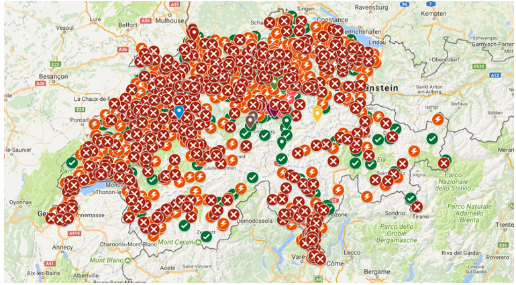
\includegraphics{Mappa uffici postali a rischio.PNG}
    \caption{Caption}
    \label{fig:my_label}
\end{figure}
\begin{figure}
    \centering
    
\includegraphics{sta per essere chiuso.PNG}
    \label{fig:my_label}
\end{figure}
Ufficio postale sta per essere chiuso.
\begin{figure}
    \centering
    
\includegraphics{a rischio dal 2020.PNG}
    \label{fig:my_label}
\end{figure}
Ufficio postale è “a rischio dal 2020”; 
si presume di che la Posta verifichi 
la chiusura di questo ufficio postale 
dopo il 2020, a meno che il legislatore 
non emani nuove direttive.
\begin{figure}
    \centering
    
\includegraphics{garantito a medio termine.PNG}
    \label{fig:my_label}
\end{figure}
Ufficio postale è “garantito a medio 
termine”; esso corrisponde ai 
criteri della Posta o del legislatore,
dunque il suo funzionamento
dovrebbe essere garantito anche 
dopo il 2020.
Il sindacato non ha una lista degli uffici che sono stati effettivamente chiusi. La Posta invece ha rilasciato una lista degli uffici che chiuderanno entro il 2020 (la lista è presente negli allegati). Secondo questa lista, in Ticino sono 48 gli uffici che nel 2017 sono stati messi in verifica di cui il 95\% molto probabilmente chiuderà. Ci sono alte probabilità che dopo il 2020 la Posta chiuderà altri uffici postali. Secondo un’analisi svolta dal sindacato in futuro potrebbero rimanere solo 10 uffici.

\subsection{Punti di accesso}

\subsubsection{Filiali in partenariato}
\subsubsection{Filiali}
\subsubsection{Servizio a domicilio}
\subsubsection{MyPost 24}
\subsubsection{Cassette delle lettere: a domicilio}
\subsubsection{Postomat}
\subsubsection{Buche delle lettere}

\subsection{Risparmi sull'accessibilità}
\subsection{Le agenzie e il servizio a domicilio}
Tra le agenzie in partenariato e gli uffici postali esistono delle sostanziali differenze nelle operazioni che i clienti possono effettuare.
\textbf{Differenze ufficio postale e filiale in partenariato}
\begin{table}[]
\begin{tabular}{ll}
\cline{1-2} \cline{4-6}
\textbf{Un ufficio postale può}                                                                                        & \textbf{Un’agenzia postale può…}                                                                                &  &  &  &  \\ \cline{1-2} \cline{4-6} 
Prendere in consegna lettere e pacchi                                                                                  & Prendere in consegna lettere e pacchi                                                                           &  &  &  &  \\
Effettuare versamenti elettronici                                                                                      & Effettuare versamenti elettronici                                                                               &  &  &  &  \\
\begin{tabular}[c]{@{}l@{}}Operazioni in contrassegno (cliente paga merce\\ ordinata all’ufficio postale)\end{tabular} & -                                                                                                               &  &  &  &  \\ \cline{4-6} 
Ritiro di atti giudiziali e di atti esecutivi                                                                          & -                                                                                                               &  &  &  &  \\
Riscuotere pagamenti                                                                                                   & \begin{tabular}[c]{@{}l@{}}Ammessi solo in parte e solo per piccoli importi\\ (fino a 500 franchi)\end{tabular} &  &  &  &  \\
Versamenti in contanti                                                                                                 & -                                                                                                               &  &  &  &  \\
Apertura conto                                                                                                         & -                                                                                                               &  &  &  &  \\
Cambio soldi (centrale per il commercio)                                                                               & -                                                                                                               &  &  &  &  \\
Identificazioni (es. aprire un conto)                                                                                  & -                                                                                                               &  &  &  &  \\
PromoPost                                                                                                              & -                                                                                                               &  &  &  &  \\
\begin{tabular}[c]{@{}l@{}}Invii in grandi quantità di clienti commerciali e\\ associazioni\end{tabular}               & Possibili, ma ad un altro prezzo                                                                                &  &  &  &  \\
Ulteriore sviluppo possibile                                                                                           & -                                                                                                               &  &  &  & 
\end{tabular}
\end{table}

\subsection{Sondaggio presso i Comuni}
Per ottenere dati concreti sul tema della chiusura degli uffici postali in Ticino ho elaborato un sondaggio con domande dirette che toccavano principalmente aspetti legati al personale, alle procedure di chiusure e alle soluzioni alternative applicate. Prima di far partire il sondaggio ho preferito farlo visionare da mie conoscenze che sono impiegate nel Comune di Riva San Vitale e altre che hanno lavorato nel Comune di Pregassona. Attraverso questi confronti ho potuto constatare che diversi Comuni non sarebbero stati in grado di rispondermi e che quindi il sondaggio avrebbe perso senso. Discutendo con i docenti siamo arrivati alla conclusione di non farlo partire nonostante l’impegno e il tempo impiegato per elaborarlo.

\subsection{La Posta come datore di lavoro}
La Posta si impegna a favore della salute e dello sviluppo personale di 62'000 collaboratori e collaboratrici. Crea un ambiente lavorativo diversificato e offre modelli di tempo di lavoro flessibile. L’azienda è stata tra i primi grandi gruppi svizzeri ad essere insignita del sigillo di qualità Friendly Work Space dalla fondazione Promozione Salute Svizzera.
\subsubsection{Modelli di tempo di lavoro moderni}
La posta pensa ai propri collaboratori proponendo modelli di lavoro individuali, offrendo se possibile e se richiesto orari di lavoro flessibili, lavoro a tempo parziale, tempo di lavoro annuale, job e top sharing oppure home office e promuove la mobilità all’interno dell’azienda.
\subsubsection{Ambiente di lavoro moderno}
L’ambiente lavorativo offerto dalla Posta permette di promuovere idee creative, progetti innovativi e un lavoro produttivo nel rispetto delle esigenze dei collaboratori.
\subsubsection{Formazione e perfezionamento}
La Posta investe nella formazione e nel perfezionamento dei propri impiegati per favorire il loro sviluppo personale e per il successo aziendale.
\subsubsection{Benefit}
Il diritto alle vacanze varia a seconda della funzione e dell’età; si aggira mediamente sulle sei settimane all’anno.
I collaboratori ottengono gratuitamente un abbonamento metà-prezzo come partecipazione agli abbonamenti per i mezzi di trasporto pubblico. Per gli abbonamenti generali gli impiegati beneficiano uno sconto del 20\%, mente per le persone in formazione presso La Posta è gratuito.
Al personale vengono offerte delle agevolazioni che spaziano dai viaggi, al tempo libero, alle assicurazioni, ai centri fitness, ecc. Essi ricevono inoltre dei buoni per prodotti o servizi della Posta o di terzi.
La Posta ha un Centro carriera, un ufficio di riferimento per questioni di riferimento e di sviluppo professionale.

\subsubsection{Incentivi ai collaboratori}
\subsubsubsection{Spirito innovativo e ricchezza di idee}
La Gestione dell’innovazione si occupa di sfruttare e portare avanti le buone idee e le conoscenze dei propri collaboratori per dare vita a nuovi modelli di business sostenibili, a nuovi prodotti o servizi, a proposte per semplificare i processi.
\subsubsubsection{Salute al primo posto}
La protezione della salute e la sicurezza sul lavoro sono principi importanti per La Posta che sensibilizza i propri dipendenti promuovendo attività di vario tipo come eventi sportivi organizzati dalla Posta (es. Bike to work, PostActivity; ecc.) o attraverso incentivi per esempio ai giovani non fumatori.
\subsubsubsection{Talento e successo}
Ogni collaboratore ai propri punti di forza e per quelli con elevato potenziale e che ottengono buone prestazioni La Posta li incentiva in modo mirato.
\subsubsubsection{Eccellenza certificata e condizioni interessanti}
La Posta è stata insignita del sigillo della qualità Friendly Work Space per il suo impegno in favore della salute dei suoi collaboratori.
Gli studenti universitari della Svizzera ritengono che La Posta sia uno dei più attrattivi datori di lavoro, anche i collaboratori tramite Kununu valutano l’azienda come una delle top companies.
“Woman Empowerment Principles” è una delle strategie del personale integrata e sottoscritta a livello internazionale dalla Posta.
Secondo un sondaggio proposto ai propri impiegati l’80\% è felice di lavorare per La Posta.


\subsection{I risparmi sul personale}
La politica di chiusura degli uffici postali ha comportato e sta tutt’ora comportando una diminuzione dei posti di lavoro negli operatori storici. In Europa sono passati da 1'190'649 nel 2004 a 771'506 nel 2011. Le condizioni di lavoro del personale hanno subito molti peggioramenti: riduzioni salariali, precariato, imposizione di tempi parziali, aumenti dei tempi parziali, aumenti dei ritmi di lavoro, stress sono ormai una caratteristica della Posta dei vari Paesi.
La messa in atto delle direttive dell’UE sulla privatizzazione e la liberalizzazione dei servizi postali avevano i seguenti tre obbiettivi:
\begin{enumerate}
    \item offrire nuove possibilità di guadagno grazie alla privatizzazione dei servizi redditizi delle telecomunicazioni;
    \item rendere redditizi i servizi deficitari (come la Posta) per poterli poi privatizzare;
    \item permettere al privato di sviluppare attività redditizie svolte in precedenza dall’azienda pubblica grazie alla liberazione del mercato.
\end{enumerate}
I risultati di questa politica, riscontrati in diversi Paesi, sono i seguenti:
\begin{enumerate}
    \item l’eliminazione del servizio pubblico che crea un pregiudizio verso i cittadini;
    \item la privatizzazione degli utili e la socializzazione delle perdite;
    \item il peggioramento delle condizioni di lavoro e la diminuzione dei posti di lavoro.
\end{enumerate}
    
\subsection{Dal punto di vista della Politica}
Nella disciplina di economia politica si è constatato che lo Stato interviene nell’economia in svariati modi per cercare di favorirla, in questo senso le possibilità di intervento da parte della politica sono le seguenti:
\begin{itemize}
    \item effettuare degli investimenti attui a rilanciare un determinato settore per renderlo attrattivo anche per gli investimenti privati;
    \item assegnare un mandato pubblico a un’azienda già esistente;
    \item costituire un’azienda statale che offra un servizio pubblico accessibile a tutti i cittadini.
    
\end{itemize}
Spesso e volentieri questi interventi portano a un iniziale monopolio da parte dello Stato di un determinato mercato che viene progressivamente aperto attraverso un processo di liberalizzazione che vede protagonisti l’azienda originaria, gli investimenti privati e le nuove aziende concorrenti.
Nel caso della Posta si è verificato un mix di queste modalità d’intervento: la politica ha inizialmente investito in questa nuova azienda assegnandole un mandato statale e sussidiandola. Il presupposto che sta alla base di questi interventi è che lo Stato agisce con la consapevolezza di non trarre guadagno dalla sua creazione e di allontanarsene progressivamente e da qui ritroviamo parte delle motivazioni per le quali oggi la Posta è una società anonima che agisce nel libero mercato che è profondamente cambiato negli ultimi anni.
La Posta ha ancora tutt’ora un mandato statale e deve comunque rendere conto delle proprie attività alle autorità politiche. Inoltre è soggetta a controlli da parte di PostCom che verifica la correttezza del suo operato.
